\label{chapter-2}
The following chapter will provide an overview of the current research on best practices when creating executable \gls{bpmn} models. First, it will discuss the motivation behind process automation and using \gls{wfms}s and the benefit it might bring to an organization. Then it will state the differences between an \gls{conceptual-bpmn}, that cannot be deployed on an \gls{wfms}, and an \gls{executable-bpmn}. Finally, this chapter will list the steps necessary to turn an \gls{conceptual-bpmn} executable.

\section{Why Automate Processes?}
Introducing an \gls{wfms} in an organization is often done to open the possibilities of automating parts of a process or even the whole process. While process automation in itself can be useful, there are some other advantages of introducing an \gls{wfms}, besides the possibility to automate certain process steps.

\subsection{Shorten Process Lifetime}
Managing processes manually requires handling tasks such as handling handovers from one entity to another. This can lead to unnecessary waiting periods between two tasks. By implementing an \gls{wfms} resource allocation and parallelization can be automated where possible to assure optimal use of process resources. \cite{gadatsch2020grundkurs}

\subsection{Reduce Process Cost}
By reducing process lifetimes and increasing productivity due to better handling of resources process costs can be reduced \cite{gadatsch2020grundkurs}. in this context, it has to be said, that due to the high price for workflow management systems the overall cost does not have to decrease necessarily after implementing an \gls{wfms} \cite{gruber2009profitability}.

\subsection{Workload Reduction}
As stated earlier, managing processes needs to be done either by an \gls{wfms} or manually which creates an additional workload for an organization. Workloads for employees executing the processes are also kept steady due to dynamic resource assignments. \cite{fundamentals}\cite{gadatsch2020grundkurs}

\subsection{Enforce Rules}
Defining the processes that are directly executed and controlled by an \gls{wfms} enables the organization to enforce the execution of the process as it is designed without giving employees room for shortcuts. Following rules and protocols regarding the process can be automated and enforcing guidelines and laws in an organization becomes easier. \cite{fundamentals}

\subsection{Create Transparency}
Using an \gls{wfms} provides insights into the actual processes that are executed in the organization. This makes it easier to determine the performance of processes by providing historical information of completed process instances and provides insight into the current status of processes that are still in progress. \cite{gadatsch2020grundkurs}

\section{Executable vs Conceptual Process Models}
Process models are inherently business-oriented as their purpose is initially to define and visualize the processes happening in an organization. Business-oriented or \gls{conceptual-bpmn} are meant to be read by domain experts and contain usually implicit information known to these experts \cite{fundamentals}. They are typically incomplete, meaning that not every possible outcome of a process is modeled. In fact, usually only the best-case scenario, also known as the \gls{happy-path}, of a process is modeled in an \gls{conceptual-bpmn} \cite{freund2019real}.\\~\\Due to their incompleteness, business-oriented models cannot be executed in an \gls{wfms} just like that but have to be turned into an \gls{executable-bpmn}. \gls{executable-bpmn} are meant for IT experts and should be a technical representation of the business process while still begin readable by domain experts. They should leave no room for interpretation as they have to contain all the information necessary for the process to be executed by an \gls{wfms}. Besides the visual information, \gls{executable-bpmn} also need to contain execution properties like interface definitions and variables that are used by the process. Those variables are called \gls{process-variables}.\cite{fundamentals} \\~\\An algorithm on how to efficiently turn an \gls{conceptual-bpmn} executable as stated in the book \textit{Fundamentals of Business Process Management} \cite{fundamentals} is described in the next section. 

\section{Making Process Models Executable}
As stated earlier, \gls{bpmn} models can not directly be executed by a \gls{bpms} but have to be converted from an \gls{conceptual-bpmn} into an \gls{executable-bpmn}. 

There are different approaches to how this conversion can take place. In \cite{fundamentals} performing such a transformation is broken down into 5 steps:
\begin{enumerate}
	\item Identify the automation boundaries
	\item Review manual tasks
	\item Complete the process model
	\item Bring the process model to an adequate granularity level
	\item Specify execution properties
\end{enumerate}

\subsection{Identify the Automation Boundaries}\label{automation}
The first step in turning an \gls{conceptual-bpmn} in an  \gls{executable-bpmn} is to identify which steps can be automated using a \gls{wfms}. 

Tasks which can inherently be automated are called \gls{automated-task}s \cite[p.~317]{fundamentals}. Taking a look at the BPMN 2.0 standard an \gls{automated-task} can be one of the following Task types:
\begin{itemize}
	\item \textbf{\gls{service-task}}: A Task that invokes a service. This service can be a webservice or application code.
	\item \textbf{\gls{send-task}}: Used to send a message to an external participant (A participant that is not part of the process).
	\item \textbf{\gls{receive-task}}: Used to receive a message from an external participant. 
	\item \textbf{\gls{script-task}}: Executes a script that can be interpreted by the \gls{wfms}.
	\item \textbf{\gls{businessrule-task}}: Executes a rule. (e.g. provides input for a business rule engine and gets the output of that calculation)
\end{itemize}

\begin{figure}[H]
	\centering
	\begin{subfigure}[b]{0.18\columnwidth}
		\centering
		
\includegraphics[width=0.9\textwidth]{graphics/service-task}
		\subcaption{Service Task}
		\label{fig:servicetask}
	\end{subfigure}
	\begin{subfigure}[b]{0.18\columnwidth}
		\centering
		
\includegraphics[width=0.9\columnwidth]{graphics/send-task}
		\subcaption{Send Task}
		\label{fig:sendtask}
	\end{subfigure}
	\begin{subfigure}[b]{0.18\columnwidth}
		\centering
		
\includegraphics[width=0.9\columnwidth]{graphics/receive-task}
		\subcaption{Receive Task}
		\label{fig:receivetask}
	\end{subfigure}
	\begin{subfigure}[b]{0.18\columnwidth}
		\centering
		
\includegraphics[width=0.9\columnwidth]{graphics/script-task}
		\subcaption{Script Task}
		\label{fig:scripttask}
	\end{subfigure}
	\begin{subfigure}[b]{0.24\columnwidth}
		
\includegraphics[width=0.675\columnwidth]{graphics/businessrule-task}
		\subcaption{Business rule Task}
		\label{fig:businessruletask}
	\end{subfigure}
	\caption{Automated tasks according to the BPMN 2.0 standard \cite{bpmnstandard}} % Remove the [...] argument if the original caption should be used in the figure list.
	\label{fig:automatedtasks} % \label has to be placed AFTER \caption (or \subcaption) to produce correct cross-references.
\end{figure}

Usually, not every step in a process can be fully automated. Processes can also have \textbf{manual tasks} and \textbf{user tasks}. While both describe activities performed by humans,\textbf{user tasks} are aided by the orchestration and resource management functionalities of a \gls{wfms} and \textbf{manual tasks} do not interact with the business process execution engine at all. 

\begin{figure}[h]
	\centering
	\begin{subfigure}[b]{0.18\columnwidth}
		\centering
		
\includegraphics[width=0.9\textwidth]{graphics/user-task}
		\subcaption{User Task}
		\label{fig:usertask}
	\end{subfigure}
	\begin{subfigure}[b]{0.18\columnwidth}
		\centering
		
\includegraphics[width=0.9\columnwidth]{graphics/manual-task}
		\subcaption{Manual Task}
		\label{fig:manualtask}
	\end{subfigure}
	\caption{Manual and user tasks according to the BPMN 2.0 standard \cite{bpmnstandard}} % Remove the [...] argument if the original caption should be used in the figure list.
	\label{fig:nonautomatedtasks} % \label has to be placed AFTER \caption (or \subcaption) to produce correct cross-references.
\end{figure}

\subsection{Review Manual Tasks}\label{manual}
As mentioned earlier manual tasks are not automated and do also happen without the aid of a \gls{wfms}. Most \gls{wfms} implement manual tasks as a pass-through activity, meaning the manual task is ignored \cite{manual-activity}\cite{manual-camunda}\cite{manual-bizagi}. To incorporate all aspects of the process into the \gls{wfms}, it is necessary to evaluate if the identified manual tasks in our \gls{bpmn}-model can be substituted by other BPMN constructs. This can be done in the following ways:
\begin{itemize}
	\item \textbf{Automate the task}: Trying to extend the current automation boundaries would be the best case scenario \gls{receive-task}. Depending on the nature of the task that is currently performed manually, this might not always be possible. 
	
	\item \textbf{Turn it into a user task}: If the task cannot be automated or the organization lacks the resources to automate the task yet, another possibility is to change the manual task into a user task. The \gls{wfms} manages task assignments and after completion, the system is notified via a worklist handler. \cite{stefanov2014business}
\end{itemize}

In the case that neither an automated task nor a user task is suitable for modeling the manual task, one might also consider isolating the task and modeling the rest of the process. If this is also not possible, due to the manual task being crucial for the expressiveness of the model, it might be reconsidered if this process can or should be considered to be executed using a \gls{wfms}\cite[p.~228]{freund2019real}

\subsection{Complete the Process Model}\label{complete}
Usually, \gls{conceptual-bpmn}s are not complete and leave out certain information that is seen as implicit knowledge or as not important by the person modeling the process. These gaps in the model might be crucial when a complete picture of the process is needed for automation. 

A common incompleteness in many conceptual models is ignoring errors and only implementing the \gls{happy-path} of a process. The \gls{happy-path} is the best-case scenario that can happen in the execution of a process. While it might be sufficient for a conceptual model, the corresponding executable BPMN model has to define what happens in case any error occurs. 

Apart from defining alternative process paths, in this step of turning a model executable, it is also necessary to model the input and output data of tasks and gateways. In the BPMN 2.0 specification this is done using \gls{data-store}s and \gls{data-object}s. 

\begin{figure}[H]
	\centering
	\begin{subfigure}[b]{0.18\columnwidth}
		\centering
		
\includegraphics[width=0.9\columnwidth]{graphics/data-store}
		\caption{Data Store} 
		\label{fig:datastore} 
	\end{subfigure}
	\begin{subfigure}[b]{0.18\columnwidth}
		\centering
		
\includegraphics[width=0.8\columnwidth]{graphics/data-object}
		\subcaption{Data Object}
		\label{fig:dataobject}
	\end{subfigure}
	\caption{Data store and data objects according to the BPMN 2.0 standard \cite{bpmnstandard}} % Remove the [...] argument if the original caption should be used in the figure list.
	\label{fig:datastoreandobject} % \label has to be placed AFTER \caption (or \subcaption) to produce correct cross-references.
\end{figure}

\subsection{Bring the Process Model to an Adequate Granularity Level}\label{granulartity}
The granularity of tasks in an \gls{conceptual-bpmn} does differ from the granularity needed in an \gls{executable-bpmn}.
As mentioned before, using an \gls{wfms} is not just about the possibility of automation, but mainly the orchestration and deciding who needs to be doing which task. \cite{freund2019real}
\\~\\Therefore consecutive tasks that are done by the same participant should be clustered together to minimize handovers that have to be unnecessarily processed by the workflow management system. \cite{fundamentals}
However, there are some exceptions to this rule:
\begin{itemize}
	\item \textbf{Tracking progress}: To know how much the process has advanced, it can be useful to split certain tasks even if they are done by the same participant. 
	\item \textbf{Handling exceptions}: If different errors and exceptions can occur for a set of tasks that is performed by the same participant, it is recommended to keep these tasks separated.
	\item \textbf{Managing resources}: Sometimes consecutive tasks are performed by participants that have the same role, but could be done by two different participants to maximize capacity. In this case, it is also recommended to dis-aggregate the task accordingly.
\end{itemize}

\subsection{Specify Execution Properties}
The final step in turning an \gls{conceptual-bpmn} executable is to specify the implementation details of our \gls{bpmn} model. While the changes performed up to this step had an impact of the graphical rendering, the execution properties are not graphically embedded into \gls{bpmn} but are encoded into the \gls{XML} specification of the BPMN-model. \cite{fundamentals} A schematic representation of the structure of \gls{bpmn} is provided in figure \ref{fig:bpmn-schema}. For an insight in the full specification of the BPMN 2.0 XML, the \gls{xml}-schema can be found on the OMG-Website\cite{BPMN-xml-spec}. 
\begin{figure}[H]
	\centering
	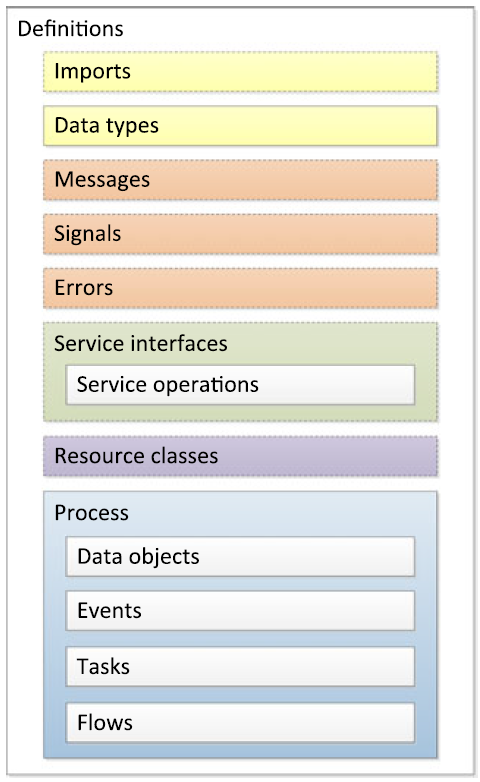
\includegraphics[width=0.3\columnwidth]{graphics/bpmn-schema}
	\caption{Structure of the BPMN format \cite{fundamentals}} 
	\label{fig:bpmn-schema} 
\end{figure}


\paragraph{Process Variables}~\\
To use data in different elements of our process, we need process variables that can be read, created, and modified during the process's execution. Every Process variable has a \textbf{data type} that can either be simple (strings, integers, doubles, booleans, dates, times, ...) or complex (composed of other types). A complex type needs to be described as an \gls{XSD}-schema file as shown in listing \ref{lst:schema-person}. 

\begin{lstlisting}[language=xml,caption={The \gls{xml}-Schema Definiton for a complex type 'person'},captionpos=b, label={lst:schema-person}]
	<xs:element name="person">
	<xs:complexType>
	<xs:sequence>
	<xs:element name="name" type="xs:string"/>
	<xs:element name="address" type="xs:string"/>
	<xs:element name="city" type="xs:string"/>
	<xs:element name="country" type="xs:string"/>
	</xs:sequence>
	</xs:complexType>
	</xs:element>
\end{lstlisting}

The corresponding complex XML object can be seen in listing \ref{lst:data-person}. 
\begin{lstlisting}[language=xml,caption={An instance of the complex type 'person'},captionpos=b,label={lst:data-person}]
	<person>
	<name>Dragana Sunaric</name>
	<address>Wiedner-Hauptstrasse 5</address>
	<city>1040 Wien</city>
	<country>Austria</country>
	</person>
\end{lstlisting}


~\\The definition of common errors, messages, and escalations that are either thrown or listened to by events and tasks are also part of the execution properties. 
\paragraph{Messages}~\\
Every BPMN element has at least an \textbf{id} that identifies the given element and a descriptive \textbf{name} of the element.\cite{bpmnstandard} Despite the properties that all BPMN elements have, messages have no additional variables that need to be set. An example of a message specification can be seen in listing \ref{lst:message}.
\begin{lstlisting}[language=xml,caption={Example for a message definition},captionpos=b,label={lst:message}]
	<message id="Message_ID" name="Message_NAME"/>
\end{lstlisting}
\paragraph{Errors}~\\
Errors additionally have an \textbf{errorCode} that specifies the given Error. Events can listen for this specific error code and trigger when it is thrown. An example error is defined in listing \ref{lst:error}.\\ 
\begin{lstlisting}[language=xml,caption={Example for a error definition},captionpos=b,label={lst:error}]
	<error id="Error_ID" name="Error_NAME" errorCode="Error_CODE"/>
\end{lstlisting}
\paragraph{Escalations}~\\
Similar to errors, escalations additionally have an \textbf{escalationCode} that can be used to listened to this escalation by events. An example for a escalation specification is shown in listing \ref{lst:escalation}.\\
\begin{lstlisting}[language=xml,caption={Example for a escalation definition},captionpos=b,label={lst:escalation}]
	<escalation id="Esc_ID" name="Esc_NAME" escalationCode="Esc_CODE"/>
\end{lstlisting}

\paragraph{Input and Output Variables}~\\
The earlier mentioned process variables are active during the whole process life-cycle. While having globally available variables has its advantages, some data used in the process might only be used in single tasks. There are even approaches to eliminate globally available process variables altogether \cite{goodbye}. For data that is only used in individual elements of the model, it is possible to define input and output values for each task. These variables are only visible within the specific task and have to be defined as an \gls{xsd}-schema file, similarly to complex process variables. \cite{fundamentals}

\paragraph{Service Tasks}~\\
Service tasks can be used to call external applications or web services. To do that, the interaction with the given service has to be defined in the process model. The called service has to provide an interface that describes the available service operations and their parameters as well as the associated return values. Service operations can be synchronous, meaning the process instance waits for the operation to return a value or error code, or asynchronous, meaning the process does not wait for a response and carries on with the process after calling the service. Based on the service interface definition, input and output variables have to be defined for the service call. The \gls{wfms} does this by copying the above-mentioned Input values of the Task into the service call and if defined, copying the output values of the service call into the output values of the service task. \cite{fundamentals}

\subsection{Apply Naming Conventions}
\label{naming}
To create readable models, it is recommended to apply naming conventions for BPMN 2.0 diagrams. While there are many suggestions for naming conventions, none is defined or recommended by the BPMN 2.0 standard \cite{bpmnstandard} itself. The following is a suggestion for naming different BPMN elements based on  \cite{freund2019real}, \cite{c}   \cite{suarez2010best} and \cite{radulian2020rethinking}. 

\paragraph{Events}~\\
Names of events should start with a business object (noun) followed by a verb. To indicate that something just happened, the verb should be in the past participle form. The noun can be specified by an adjective in front. Examples of good event names: 
\begin{itemize}
	\item \textit{order delivered}
	\item \textit{Large order delivered}
\end{itemize}

\paragraph{Tasks}~\\
Tasks should be named starting with a verb and followed by a business object (noun). The object can be specified using an adjective. If needed, the task name can also answer how the task will be accomplished by appending an explanation to the task name. Examples of good task names:
\begin{itemize}
	\item \textit{deliver order}
	\item \textit{deliver large order}
	\item \textit{deliver large order with truck}
\end{itemize}

\paragraph{Gateways}~\\
Gateways only need to be named if they are divergent exclusive gateways. Divergent exclusive gateways should consist of at least a noun followed by a verb and a question mark to indicate what is evaluated at this gateway. Alternatively, a whole question can be asked. Examples of good gateway labels:
\begin{itemize}
	\item \textit{order delivered?}
	\item \textit{was order delivered in time?}
\end{itemize}

\paragraph{Sequence Flows}~\\
Sequence flows only need to be named if they come out of diverging Event-based, exclusive, or inclusive gateways. Sequence flows that follow one of those gateways should have labels that indicate the outcome of the gateway's condition. 

\paragraph{General Rules}~\\
All tasks, events, and gateways should have a label. Sequence flows should have a label if they leave an exclusive, inclusive, or event-based gateway. Generally, the naming convention should be in it consistent and for readability, it is recommended to avoid long names. As a rule of thumb, having labels that are no longer than 5 words is recommended\cite{fundamentals}. 